\section{Experimento 1}

Para este experimento haremos uso de nuestra propia computadora, la cual conectaremos al generador de funciones para controlarlo mediante un script en Python. Para ello primero deberemos realizar las siguientes cosas:\\

Se instalo la librería picocom, con la cual podremos comunicarnos con el generador de funciones mediante un puerto serial.\\

Luego teniendo el generador encendido y conectado a la computadora mediante un cable USB, abrimos una terminal y ejecutamos el siguiente comando:\\

\begin{verbatim}
sudo picocom -b 9600 /dev/ttyUSB0
\end{verbatim}

Con dicho comando nos conectamos al generador de funciones mediante el puerto serial, y podremos enviarle comandos para controlarlo.\\

En un primer paso le mandaremos el comando *IDN?* para que nos devuelva el nombre del generador de funciones, y así verificar que la comunicación se haya establecido correctamente.\\

\begin{figure}[H]
    \centering
    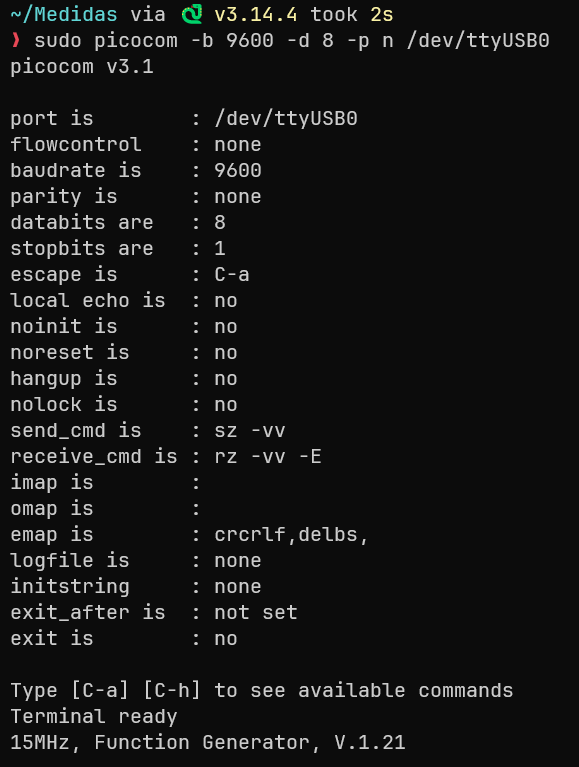
\includegraphics[width=0.4\textwidth]{images/terminal.png}
    \caption{Respuesta del generador de funciones al comando *IDN?*}
\end{figure}

Como se puede observar en la figura, el generador de funciones nos devuelve sus datos y el ancho de banda, lo cual nos indica que la comunicación se estableció correctamente.\\

Para continuar con el trabajo ahora crearemos un script en Python que nos permita controlar el generador de funciones mediante comandos. Para ello primero importamos la librería pyserial, la cual nos permite comunicarnos con el puerto serial.\\

El script que creamos es el siguiente:\\

\begin{lstlisting}[
    language=Python,
    basicstyle=\scriptsize\ttfamily,
    keywordstyle=\color{blue!75!black},
    stringstyle=\color{orange!80!black},
    commentstyle=\color{green!45!black},
    emph={serial,SerialException},
    emphstyle=\color{cyan!60!black},
    numbers=left,
    numberstyle=\tiny\color{gray},
    numbersep=6pt,
    frame=single,
    framerule=0.3pt,
    rulecolor=\color{gray!50},
    backgroundcolor=\color{gray!8},
    showstringspaces=false,
    breaklines=true,
    columns=fullflexible,
    literate={á}{{\'a}}1 {é}{{\'e}}1 {í}{{\'i}}1 {ó}{{\'o}}1 {ú}{{\'u}}1 {ñ}{{\~n}}1
]
import serial
import time


PUERTO = '/dev/ttyUSB0'  
BAUD_RATE = 9600

# Saltos definidos en el procedimiento
frecuencias_barrido = [1000, 2000, 5000, 10000, 20000, 50000, 100000]

try:
    gf = serial.Serial(PUERTO, BAUD_RATE, timeout=1)
    print(f"[*] Conectado al generador en {PUERTO}.")

    comandos_iniciales = [
        "SOUR:FUNC SIN\n",
        "SOUR:VOLT 5.0\n",
        "SOUR:VOLT:OFFS 0\n",
        "OUTP ON\n"
    ]
    
    for cmd in comandos_iniciales:
        gf.write(cmd.encode('ascii'))
        time.sleep(0.1)

    print("[*] Configuración inicial aplicada (Senoidal, 5Vpp, Offset 0V).")
    print("[*] Iniciando barrido con intervención del operador (Opción B).")


    for freq in frecuencias_barrido:

        input(f"\n[?] Presiona ENTER para ajustar la frecuencia a {freq} Hz...")
        
        comando_freq = f"SOUR:FREQ {freq}\n"
        gf.write(comando_freq.encode('ascii'))
        print(f" ---> Generando {freq} Hz. Observa el osciloscopio y toma nota.")

    print("\n[*] Barrido finalizado con éxito.")

except serial.SerialException as e:
    print(f"[!] Error de puerto serie: {e}")
finally:
    if 'gf' in locals() and gf.is_open:
        gf.close()
\end{lstlisting}

Al inicio del codigo definimos el puerto y la velocidad de comunicación, luego creamos una lista con las frecuencias que queremos barrer.\\

Luego abrimos el puerto serial y enviamos los comandos iniciales para configurar el generador de funciones.\\

A continuación, realizamos un barrido de frecuencias, donde el operador debe presionar ENTER para avanzar a la siguiente frecuencia.\\

Finalmente cerramos el puerto serial.\\

Cuando el codigo esta en funcionamiento, el operador debe observar la señal en el osciloscopio y tomar nota de los resultados.\\

Por otro lado configuramos el generador de funciones para que este tenga 9600 baudios

\begin{figure}[H]
    \centering
    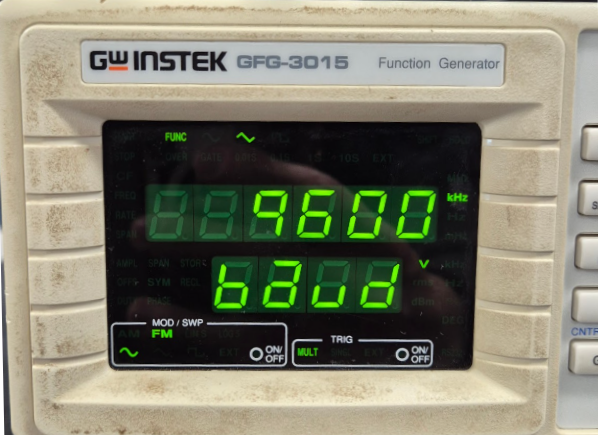
\includegraphics[width=0.4\textwidth]{images/osciloscopio.png}
    \caption{Configuración del generador de funciones a 9600 baudios}
\end{figure}

Utilizaremos una placa de pruebas representada por el siguiente esquema por la cual mediremos la señal y el potencial eC en el osciloscopio.\\

\begin{figure}
    \centering
    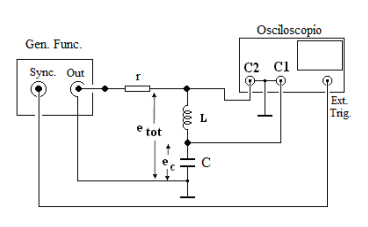
\includegraphics[width=0.4\textwidth]{images/esquema.png}
    \caption{Esquema de la placa de pruebas}
\end{figure}

Ahora configuramos el osciloscopio para que muestre la señal de manera correcta, y cambiamos el modo al Matemático para poder observar la señal de manera más clara.\\

Para ello seleccionamos FFT, en el modo de ventana Hanning, y centramos la señal para luego aplicar el x10 en el eje Y.\\

Ahora iniciamos el barrido de frecuencias, y observamos la señal en el osciloscopio.\\

\begin{figure}
    \centering
    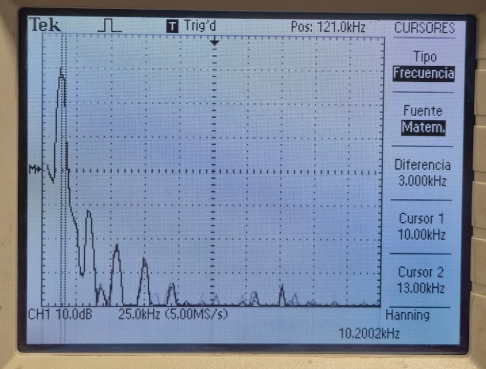
\includegraphics[width=0.4\textwidth]{images/exp1.png}
    \caption{Configuración del osciloscopio en modo Matemático}
\end{figure}

Vemos que a la frecuencia de 10kHz la señal se encuentra en su punto máximo.\\

Tocamos un poco el generador manualmente para encontrar el punto de resonancia, y vemos que se encuentra en 10.2kHz.

\begin{figure}[H]
    \centering
    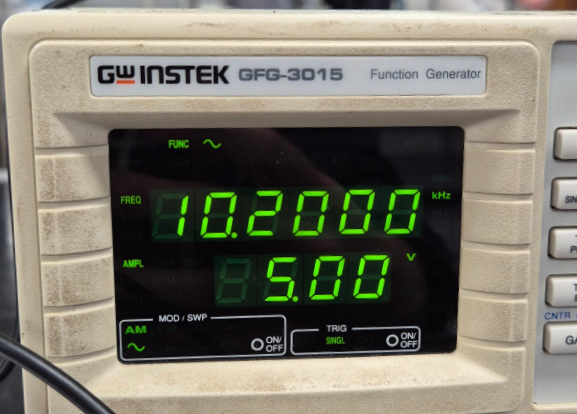
\includegraphics[width=0.4\textwidth]{images/exp2.png}
    \caption{Señal en el osciloscopio a 10.2kHz}
\end{figure}

Ahora modificamos el barrido para llegar a +3dB y -3dB, para que lleguemos a ese punto nuestra amplitud debe ser de 19.6dB ya que en el punto de resonancia la amplitud es de 22.6dB.\\

El barrido que utilizaremos es desde 8kHz hasta 14kHz, con saltos de 200Hz cuando esté entre 9kHz y 12kHz, y de 500Hz cuando esté fuera de ese rango.\\

\begin{figure}[H]
    \centering
    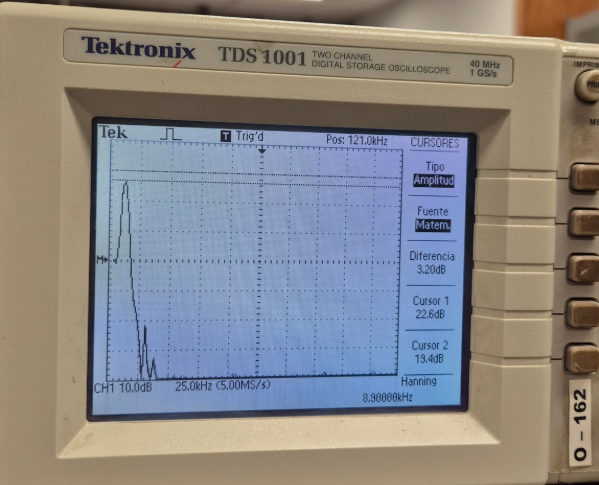
\includegraphics[width=0.4\textwidth]{images/exp3.png}
    \caption{Señal en el osciloscopio a +3dB y -3dB}
\end{figure}

\begin{figure}[H]
    \centering
    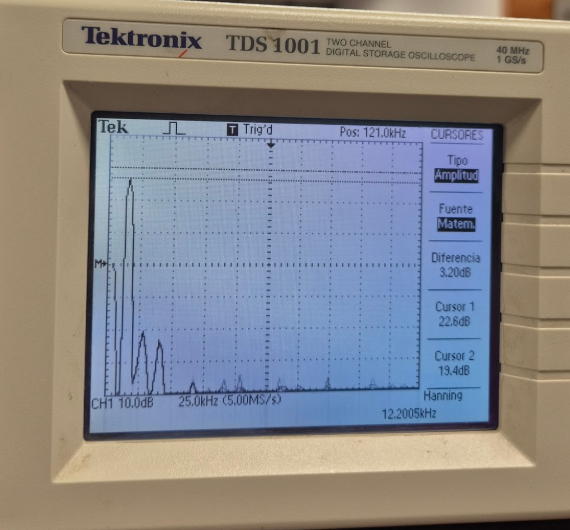
\includegraphics[width=0.4\textwidth]{images/exp4.png}
    \caption{Señal en el osciloscopio a +3dB y -3dB}
\end{figure}

Vemos que en el punto de +3dB la frecuencia es de 12.2kHz y en el punto de -3dB la frecuencia es de 9kHz.\\


Como ultimo paso compararemos los resultados obtenidos con los calculados, para ello utilizaremos la siguiente formula:\\

\begin{equation*}
    f_r = \frac{1}{2\pi\sqrt{LC}}
\end{equation*}

Reemplazando los valores de L = 20mH y C = 7nF obtenemos:

\begin{equation*}
    f_r = \frac{1}{2\pi\sqrt{20mH * 7nF}} = 13.45kHz
\end{equation*}

Vemos que el valor calculado es cercano al medido de 10.2kHz, y la diferencia se debe a que los valores de L y C no son exactos, sino que tienen una tolerancia de 5\% y 10\% respectivamente.\\